\documentclass[10pt,xcolor=pdflatex,hyperref={unicode}]{beamer}
\usepackage{newcent}
\usepackage[utf8]{inputenc}
\usepackage[czech]{babel}
\usepackage[T1]{fontenc}
\usepackage{hyperref}
\usepackage{fancyvrb}
\usepackage{tabularx}
\usepackage{longtable}
\usepackage{makecell}
\usepackage{numprint}\usepackage{textcomp}
\usepackage{appendixnumberbeamer}
\usetheme{FIT}

%%%%%%%%%%%%%%%%%%%%%%%%%%%%%%%%%%%%%%%%%%%%%%%%%%%%%%%%%%%%%%%%%%
\title[Diplomová práce]{Realistické zobrazování voxelových scén v reálném čase}

\author[]{Bc. Petr Flajšingr}

\institute[]{Brno University of Technology, Faculty of Information Technology\\
Bo\v{z}et\v{e}chova 1/2. 612 66 Brno - Kr\'alovo Pole\\
xflajs00@fit.vutbr.cz}

%\institute[]{Fakulta informačních technologií
%Vysokého učení technického v Brně\\
%Bo\v{z}et\v{e}chova 1/2. 612 66 Brno - Kr\'alovo Pole\\
%login@fit.vutbr.cz}

% České logo - Czech logo
% beamerouterthemeFIT.sty řádek 9: fitlogo1_cz

%\date{January 1, 2016}
\date{\today}
%\date{} % bez data / without date

%%%%%%%%%%%%%%%%%%%%%%%%%%%%%%%%%%%%%%%%%%%%%%%%%%%%%%%%%%%%%%%%%%

\begin{document}

\frame[plain]{\titlepage}

\begin{frame}\frametitle{Zadání}
    \begin{center}
        Realistické zobrazování voxelových scén v reálném čase
        
        \textit{Real-Time Photorealistic Rendering of Voxel Scenes}
        \bigbreak
        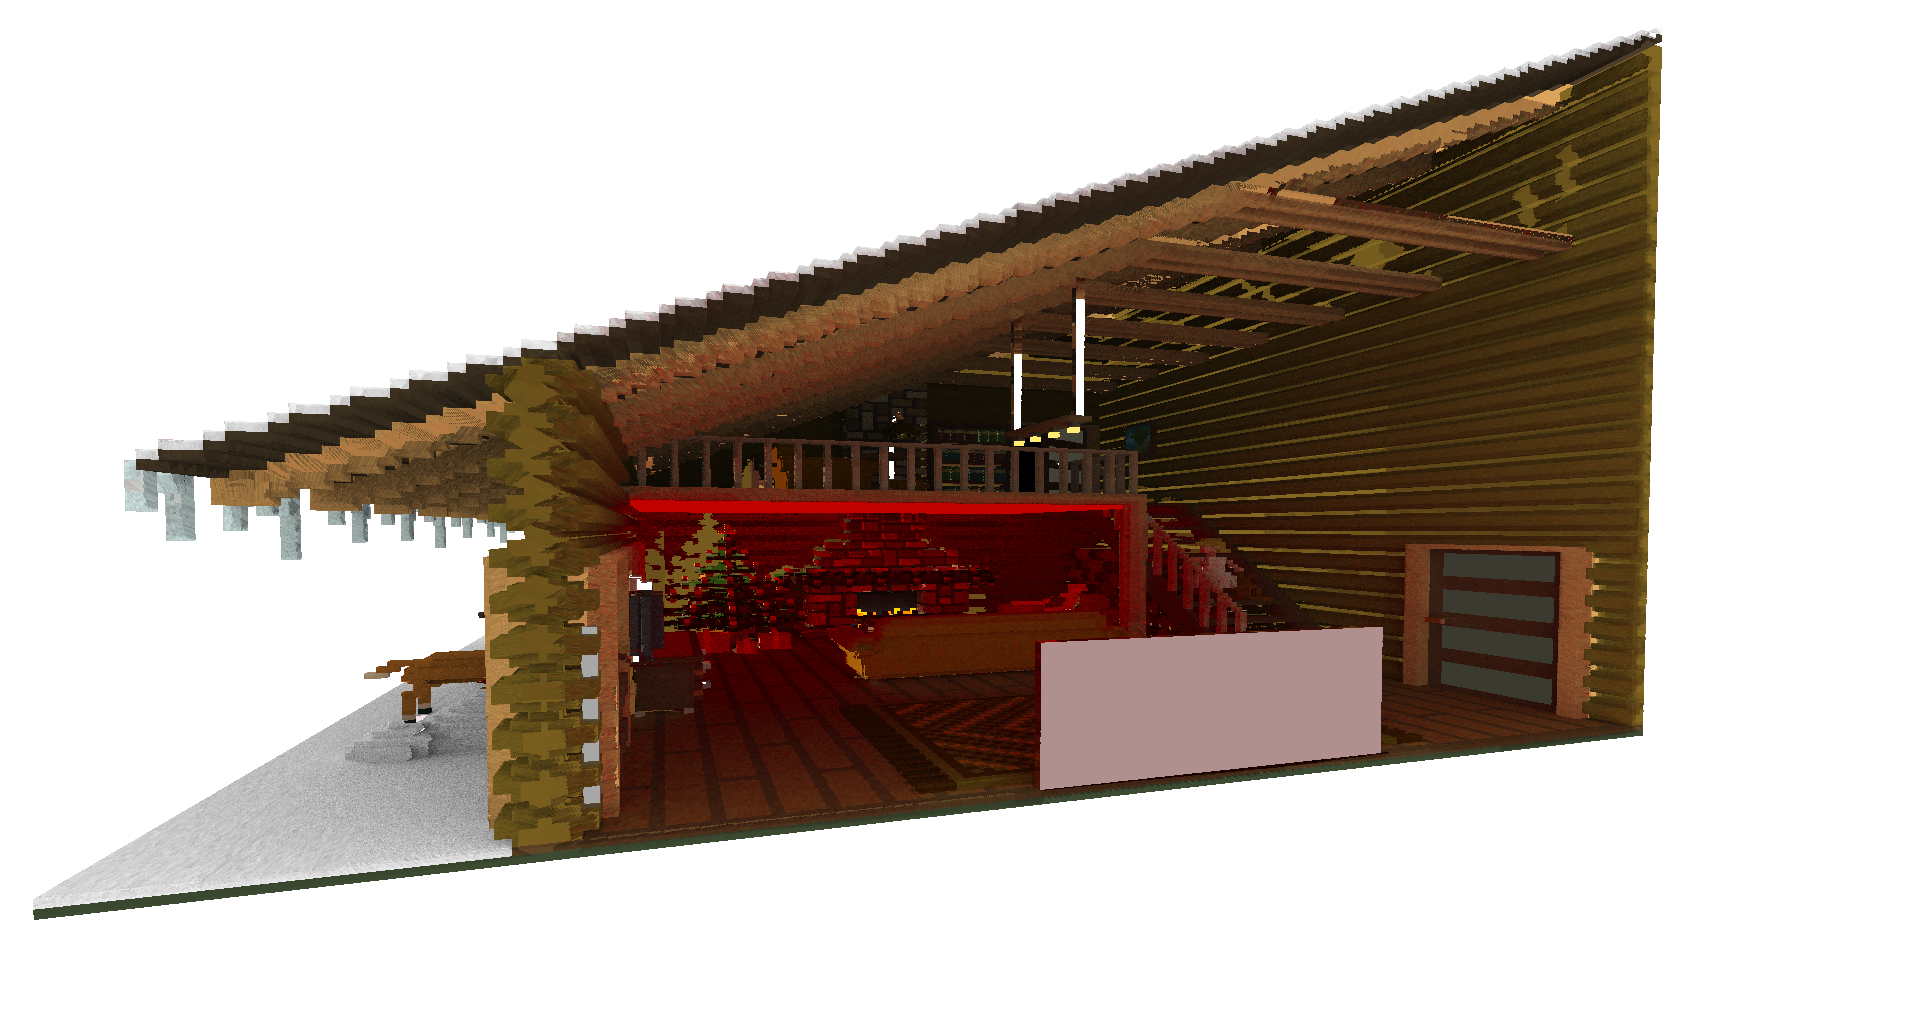
\includegraphics[width=\textwidth]{img/render1.png}%
    \end{center}
\end{frame}

\begin{frame}\frametitle{Cíl}
    \begin{columns}
        \hspace{.4cm}
        \begin{column}{0.5\textwidth}
            \textbf{Studium}
            \begin{itemize}
                \item Vulkan API
                \item Metody reprezentace a vykreslování voxelových dat
            \end{itemize}
        \end{column}
        \begin{column}{0.5\textwidth}
            
\includegraphics[scale=0.16]{img/Vulkan.png}
        \end{column}
    \end{columns}
    
    \bigbreak
    \bigbreak
    
    \textbf{Důležité články} \\
    \textit{Efficient Sparse Voxel Octrees}
    \begin{itemize}
        \item Reprezentace voxelových dat
    \end{itemize}
    \textit{Real-Time Global Illumination using Precomputed Light Field Probes}
    \begin{itemize}
        \item Globální osvětlení
    \end{itemize}
\end{frame}

\begin{frame}\frametitle{Reprezentace modelů ve scéně}
    \begin{itemize}
        \item Sparse voxel octree -- modely
        \item Bounding volume hierarchy -- scéna
    \end{itemize}
    
\includegraphics[scale=0.8]{img/scene_structure.png}%
\end{frame}

\begin{frame}\frametitle{Výpočet průsečíku se scénou}
    \begin{itemize}
        \item Implicitní řazení obalových těles podle vzdálenosti
        \item Octree ray marching pouze v kandidátních uzlech
    \end{itemize}
    \begin{column}{\textwidth}
        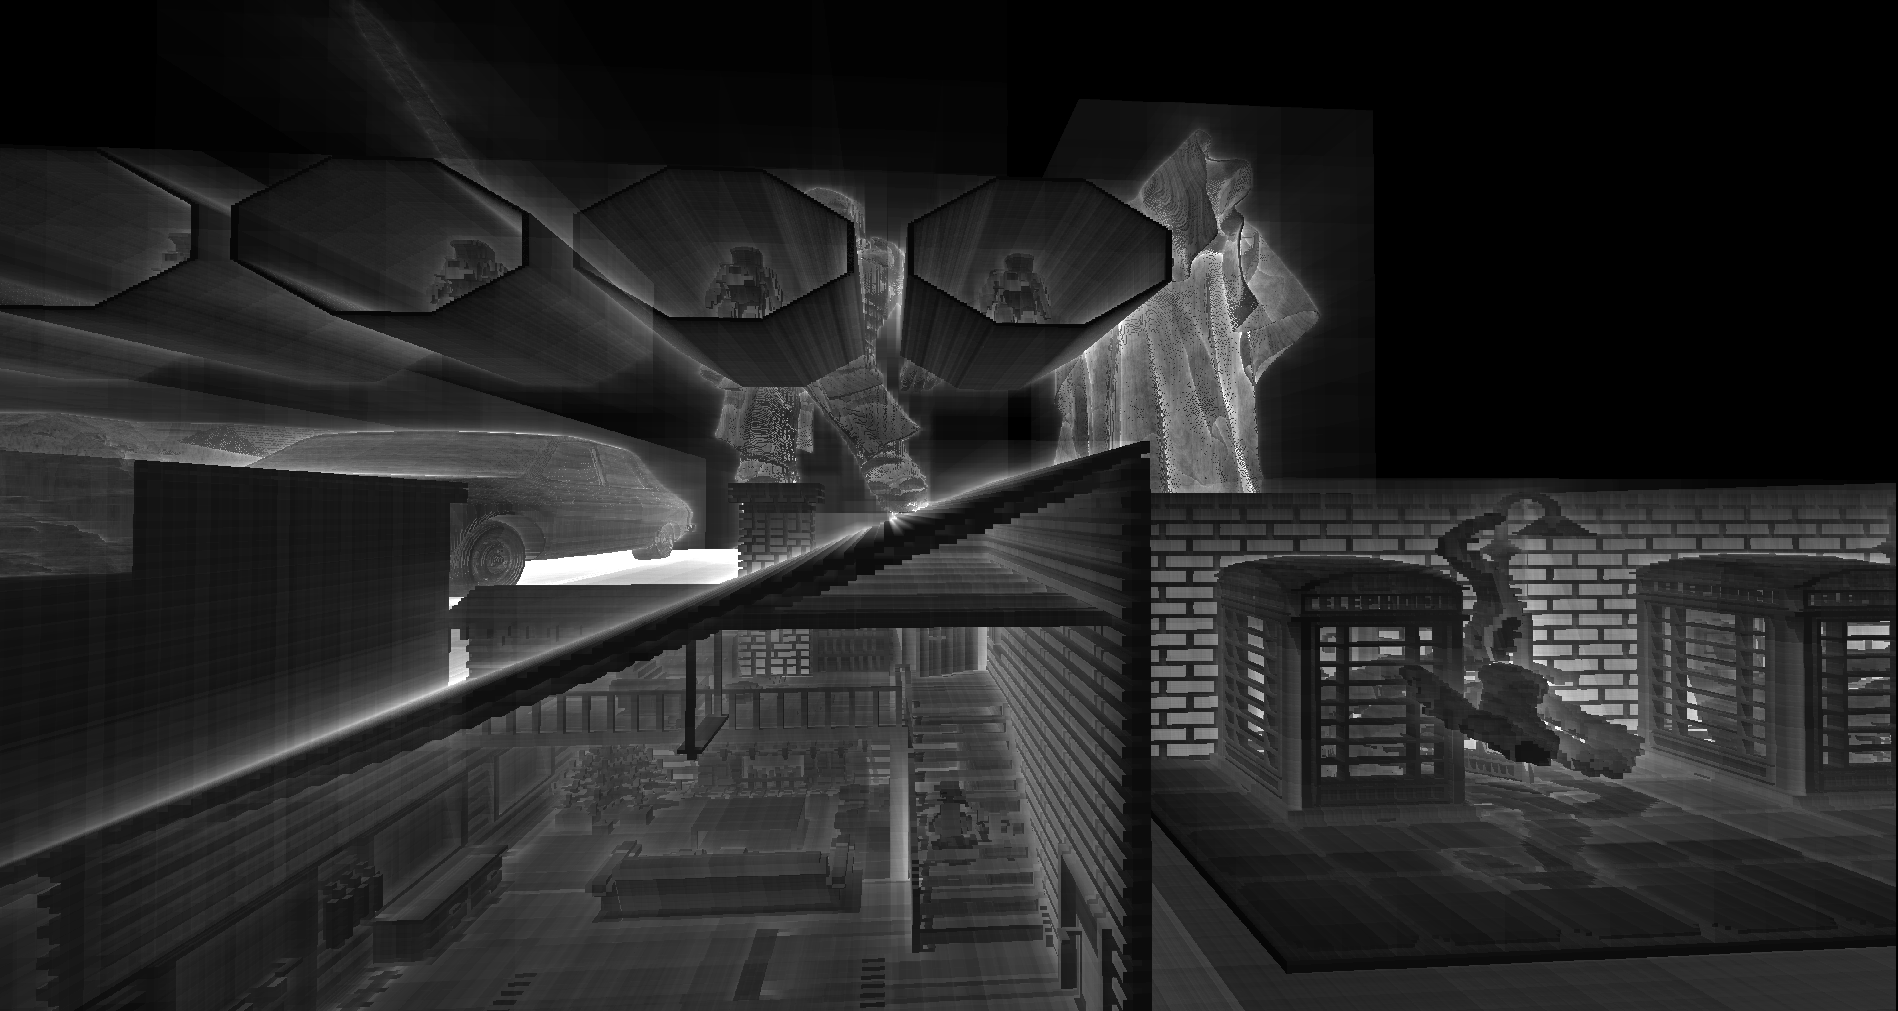
\includegraphics[width=\textwidth]{img/bvh_iter.png}
    \end{column}
\end{frame}

\begin{frame}\frametitle{Sondy světelného pole}
    \begin{itemize}
        \item Umístěny ve scéně v mřížce
        \item Scéna vykreslena z jejich pohledu
        \item Sledování paprsku metodou podobnou rasterizaci
    \end{itemize}
    \begin{column}{0.5\textwidth}
        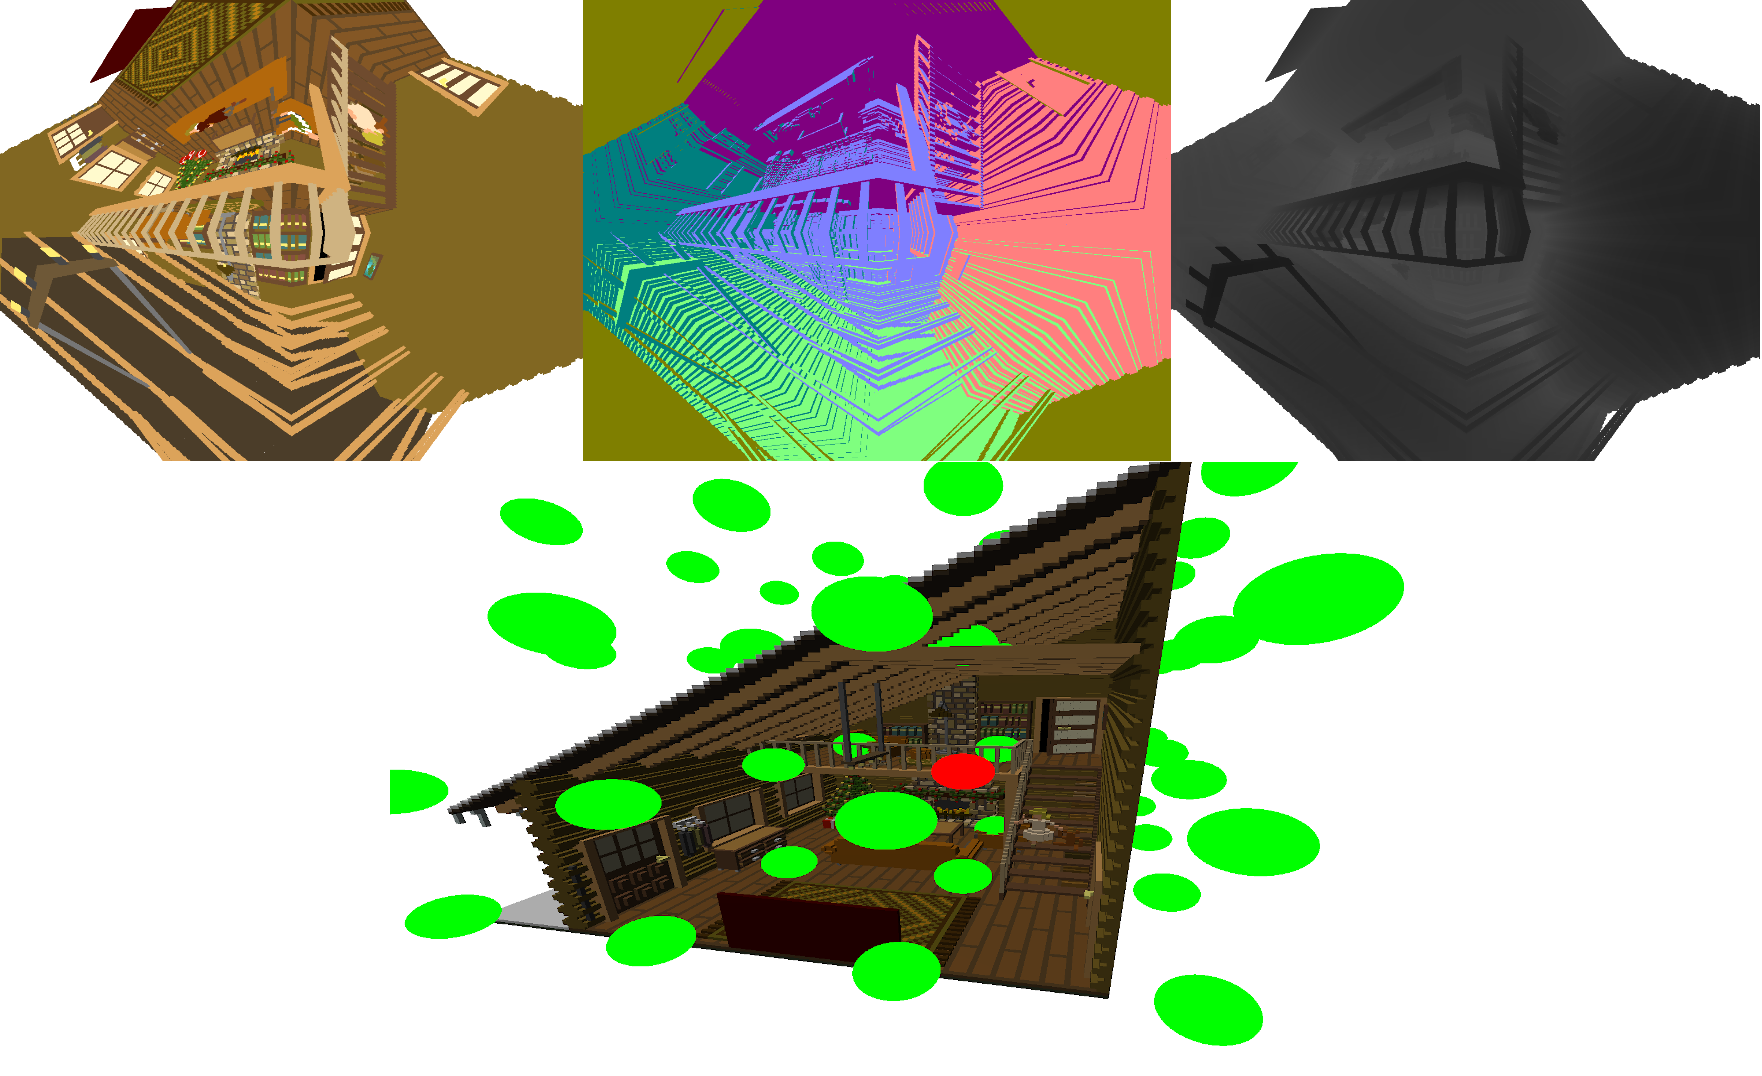
\includegraphics[width=\textwidth]{img/probe_with_scene.png}
    \end{column}
    \begin{column}{0.5\textwidth}
        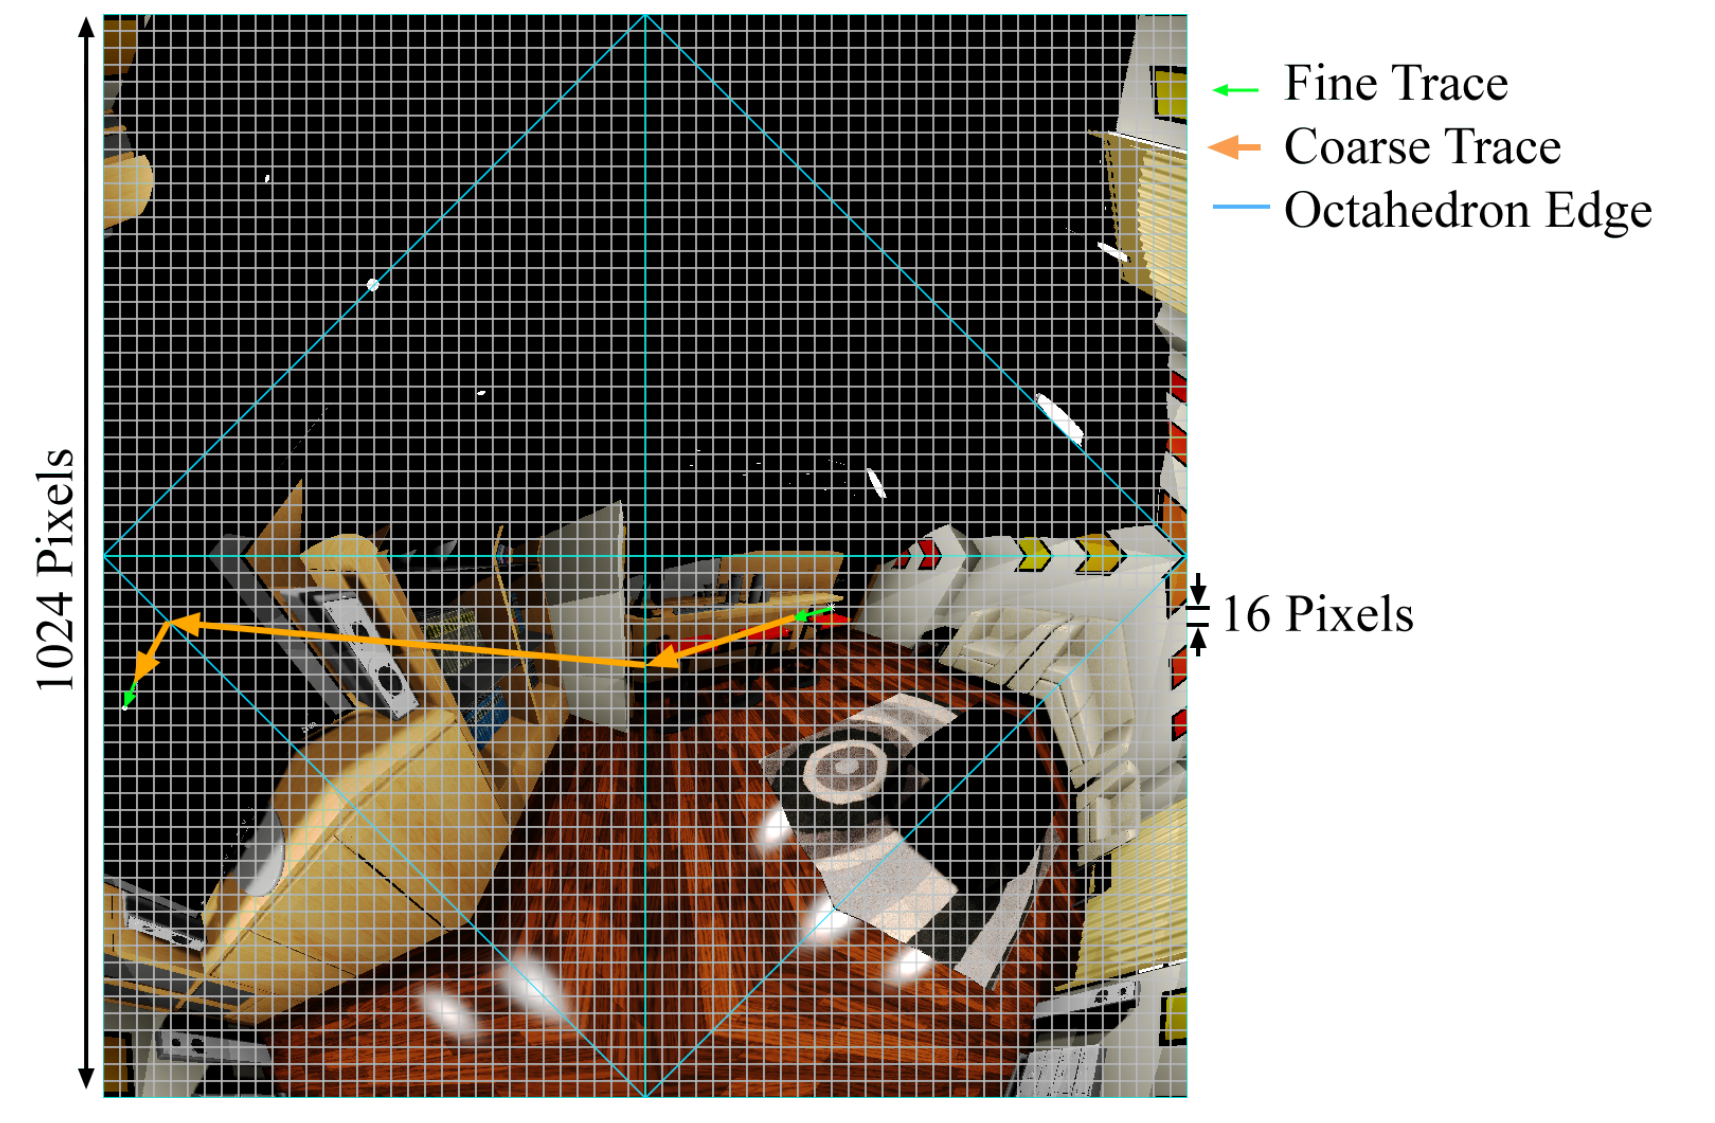
\includegraphics[width=\textwidth]{img/lfp_trace.png}
    \end{column}
\end{frame}

\begin{frame}\frametitle{Sondy světelného pole - primární paprsky}
    \begin{column}{\textwidth}
        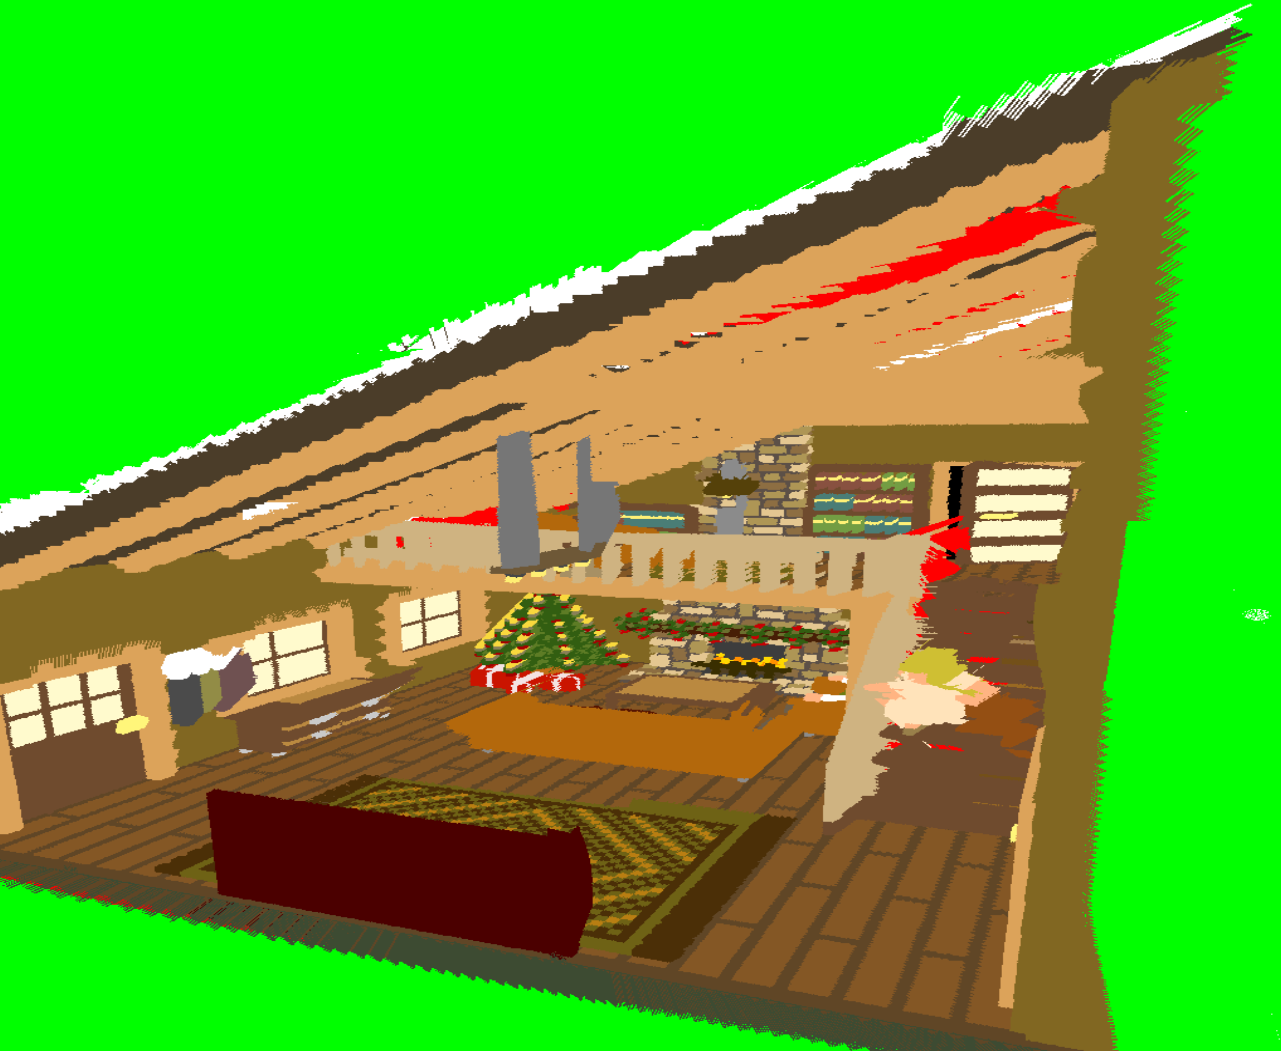
\includegraphics[width=\textwidth]{img/probe_scene_render.png}
    \end{column}
\end{frame}

\begin{frame}\frametitle{Před-vypočtené nepřímé osvětlení}
    \begin{column}{\textwidth}
        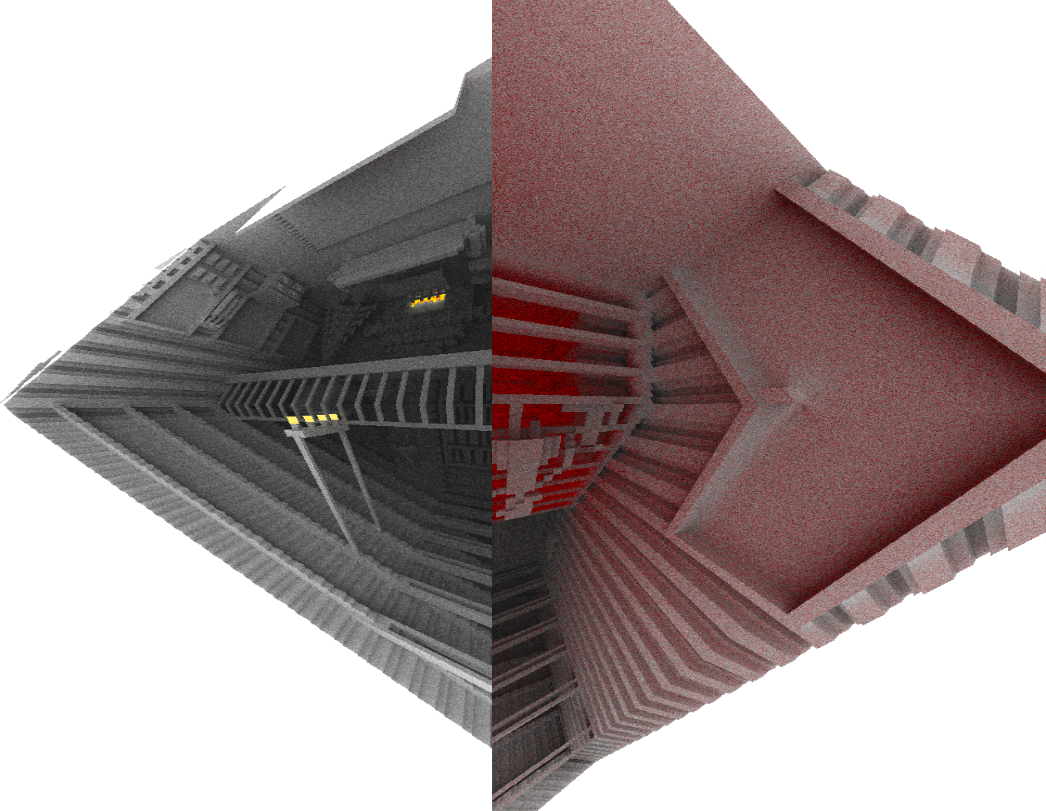
\includegraphics[width=\textwidth]{img/indirect_probe.png}
    \end{column}
\end{frame}

\begin{frame}\frametitle{Konečný vykreslovací řetězec}
    \begin{enumerate}
        \item Výpočet průsečíku v octree, uložení data materiálu a pozice
        \item Dohledání vlivu nepřímého osvětlení pro fragmenty
    \end{enumerate}
    \begin{column}{\textwidth}
        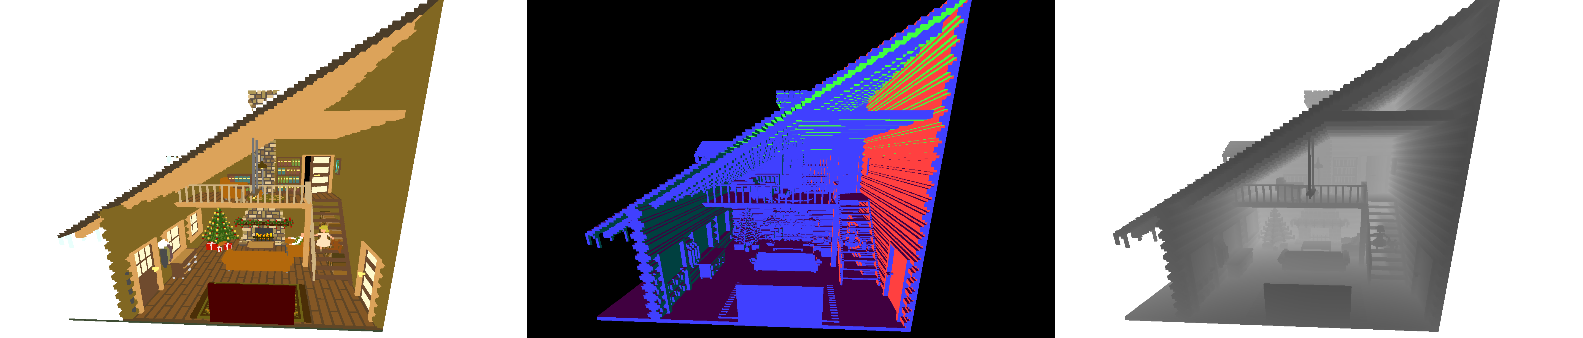
\includegraphics[width=\textwidth]{img/gbuffer_render.png}
    \end{column}
\end{frame}

\begin{frame}\frametitle{Paměťová náročnost}
        \begin{table}[H]
        	\centering
        	\begin{tabular}{r|r}
        		%\hline
        		\multicolumn{1}{c|}{hloubka stromu} & \multicolumn{1}{c}{obsazená paměť {[}B{]}} \\ \Xhline{3\arrayrulewidth}
        		1                                    & 4                                         \\ %\hline
        		2                                    & 36                                        \\ %\hline
        		3                                    & 292                                       \\ %\hline
        		4                                    & 2340                                      \\ %\hline
        		5                                    & 18724                                     \\ %\hline
        		6                                    & 149796                                    \\ %\hline
        	\end{tabular}
        \end{table}
        \begin{itemize}
            \item Příklad reálného modelu: 11 úrovní, \numprint{1050202} voxelů, 8.5 MB
            \item Příklad scény: \textasciitilde \numprint{12000000} voxelů, 741.5 MB
            \item Sonda zabírá 8.4 MB -- pro 4x4x4 tedy \textasciitilde 500 MB
        \end{itemize}
\end{frame}

\begin{frame}\frametitle{Rychlost vykreslování}
    \begin{column}{\textwidth}
        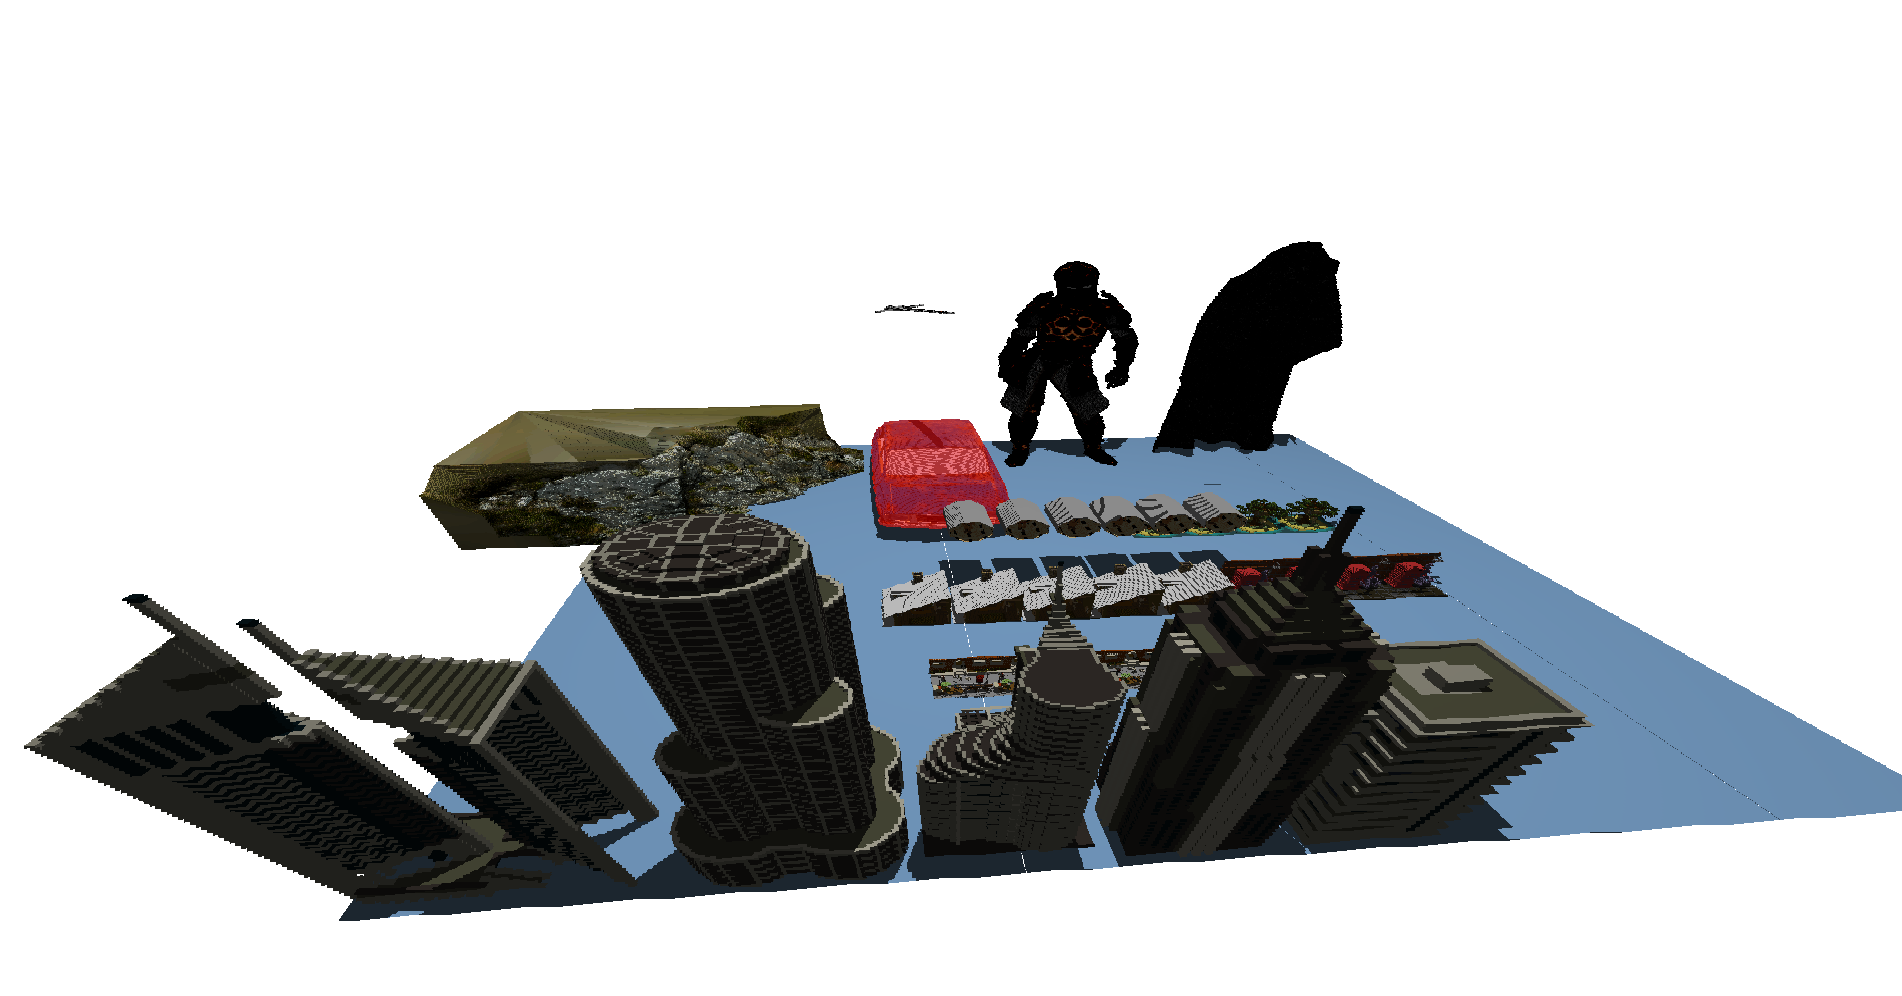
\includegraphics[width=\textwidth]{img/big_scene.png}
    \end{column}
    \begin{itemize}
        \item 12M voxelů
        \item 36 uzlů
        \item 180 fps bez stínů, 140 se stíny
    \end{itemize}
\end{frame}

\begin{frame}\frametitle{Knihovny vytvořené v rámci projektu}
    \begin{column}{0.5\textwidth}
        \begin{itemize}
            \item \texttt{pf\_common} -- obecné funkce, geometrie...
            \item \texttt{pf\_glfw\_vulkan} -- zjednodušení práce s Vulkan a GLFW, mainloop...
            \item \texttt{pf\_imgui} -- retained mode wrapper pro Dear ImGui
        \end{itemize}
    \end{column}
    \begin{column}{0.5\textwidth}
        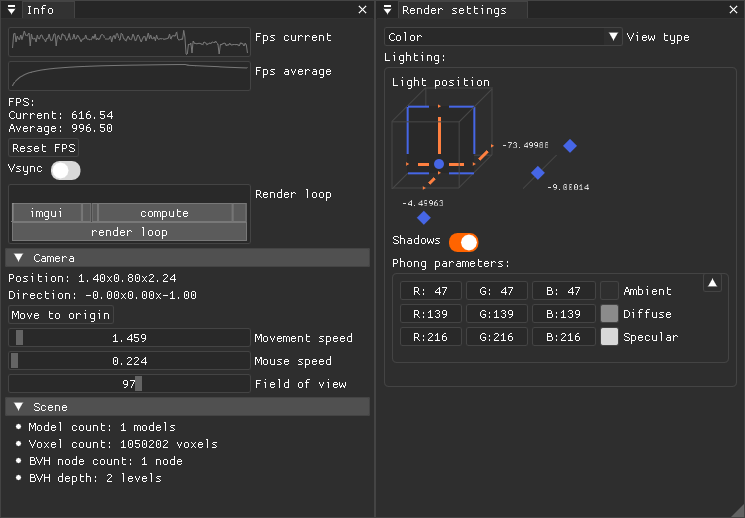
\includegraphics[width=\textwidth]{img/pf_imgui.png}
    \end{column}
\end{frame}

\begin{frame}\frametitle{Demonstrační aplikace}
    \begin{column}{\textwidth}
        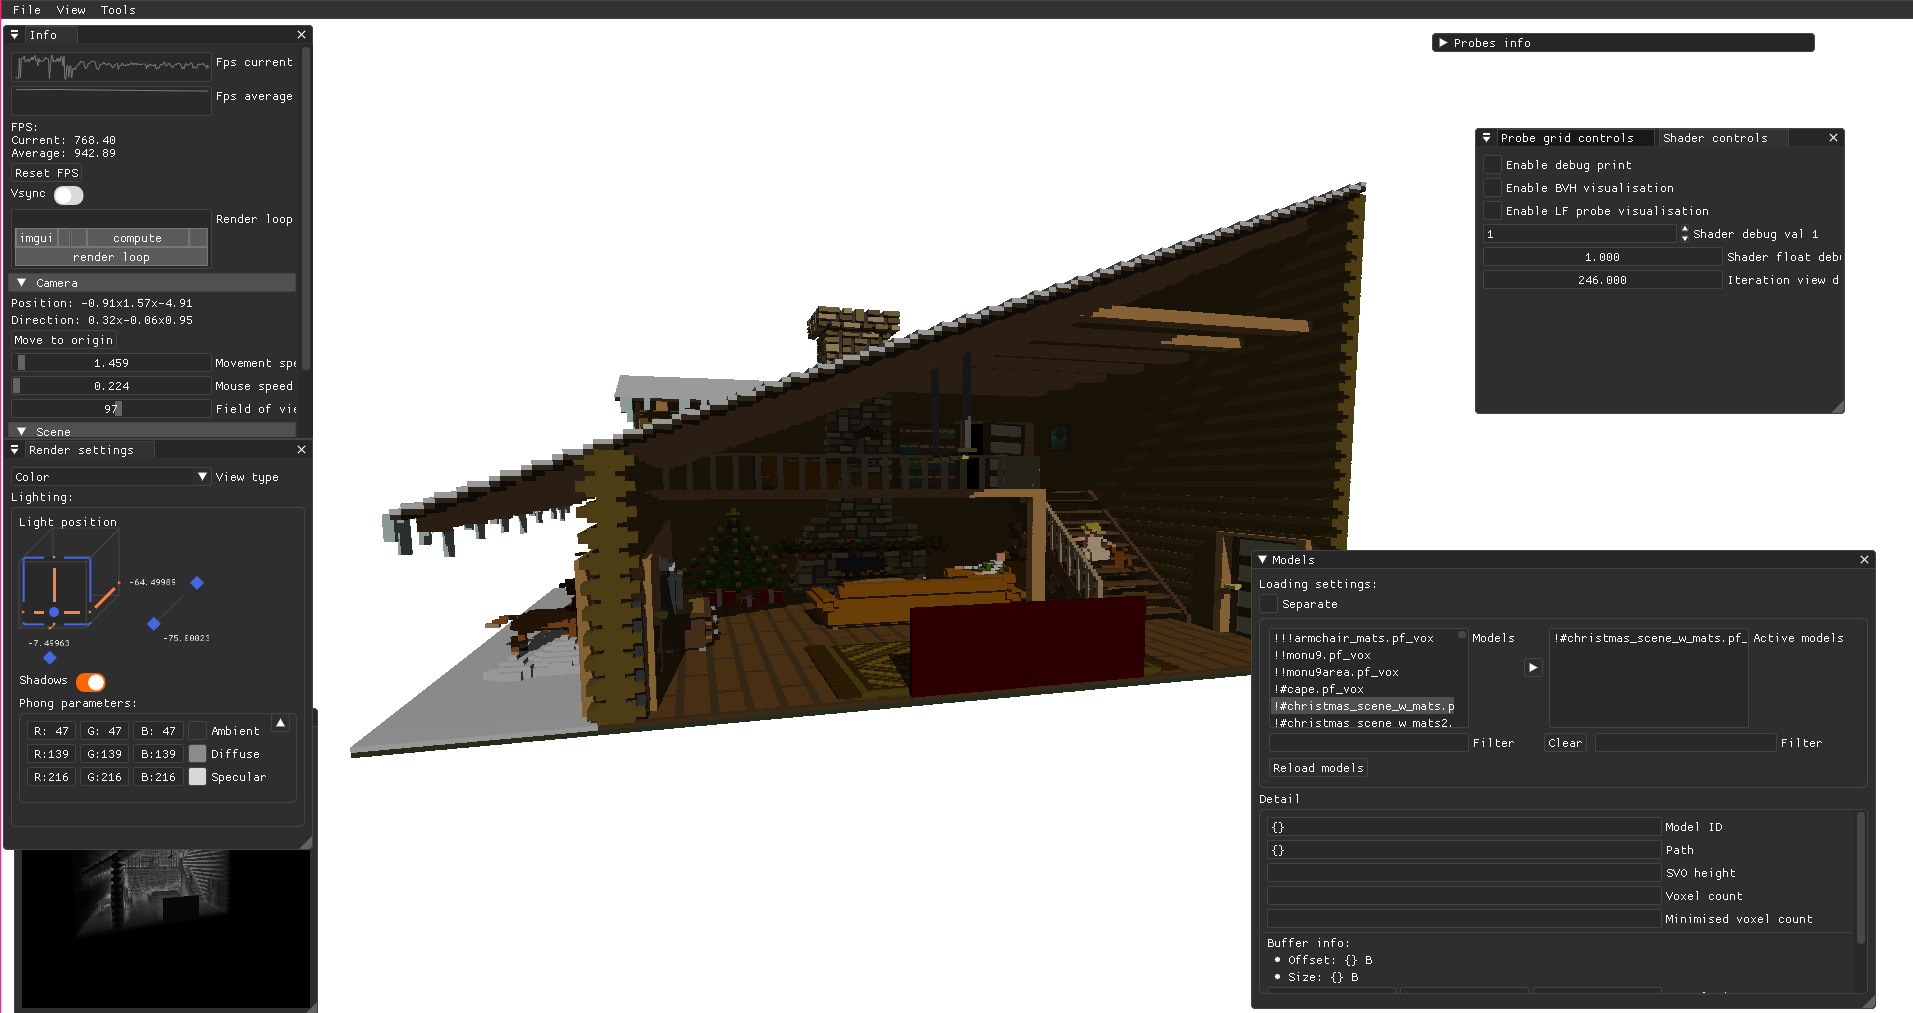
\includegraphics[width=\textwidth]{img/app.png}
    \end{column}
\end{frame}

\appendix


\begin{frame}\frametitle{Výsledky}
    \begin{column}{\textwidth}
        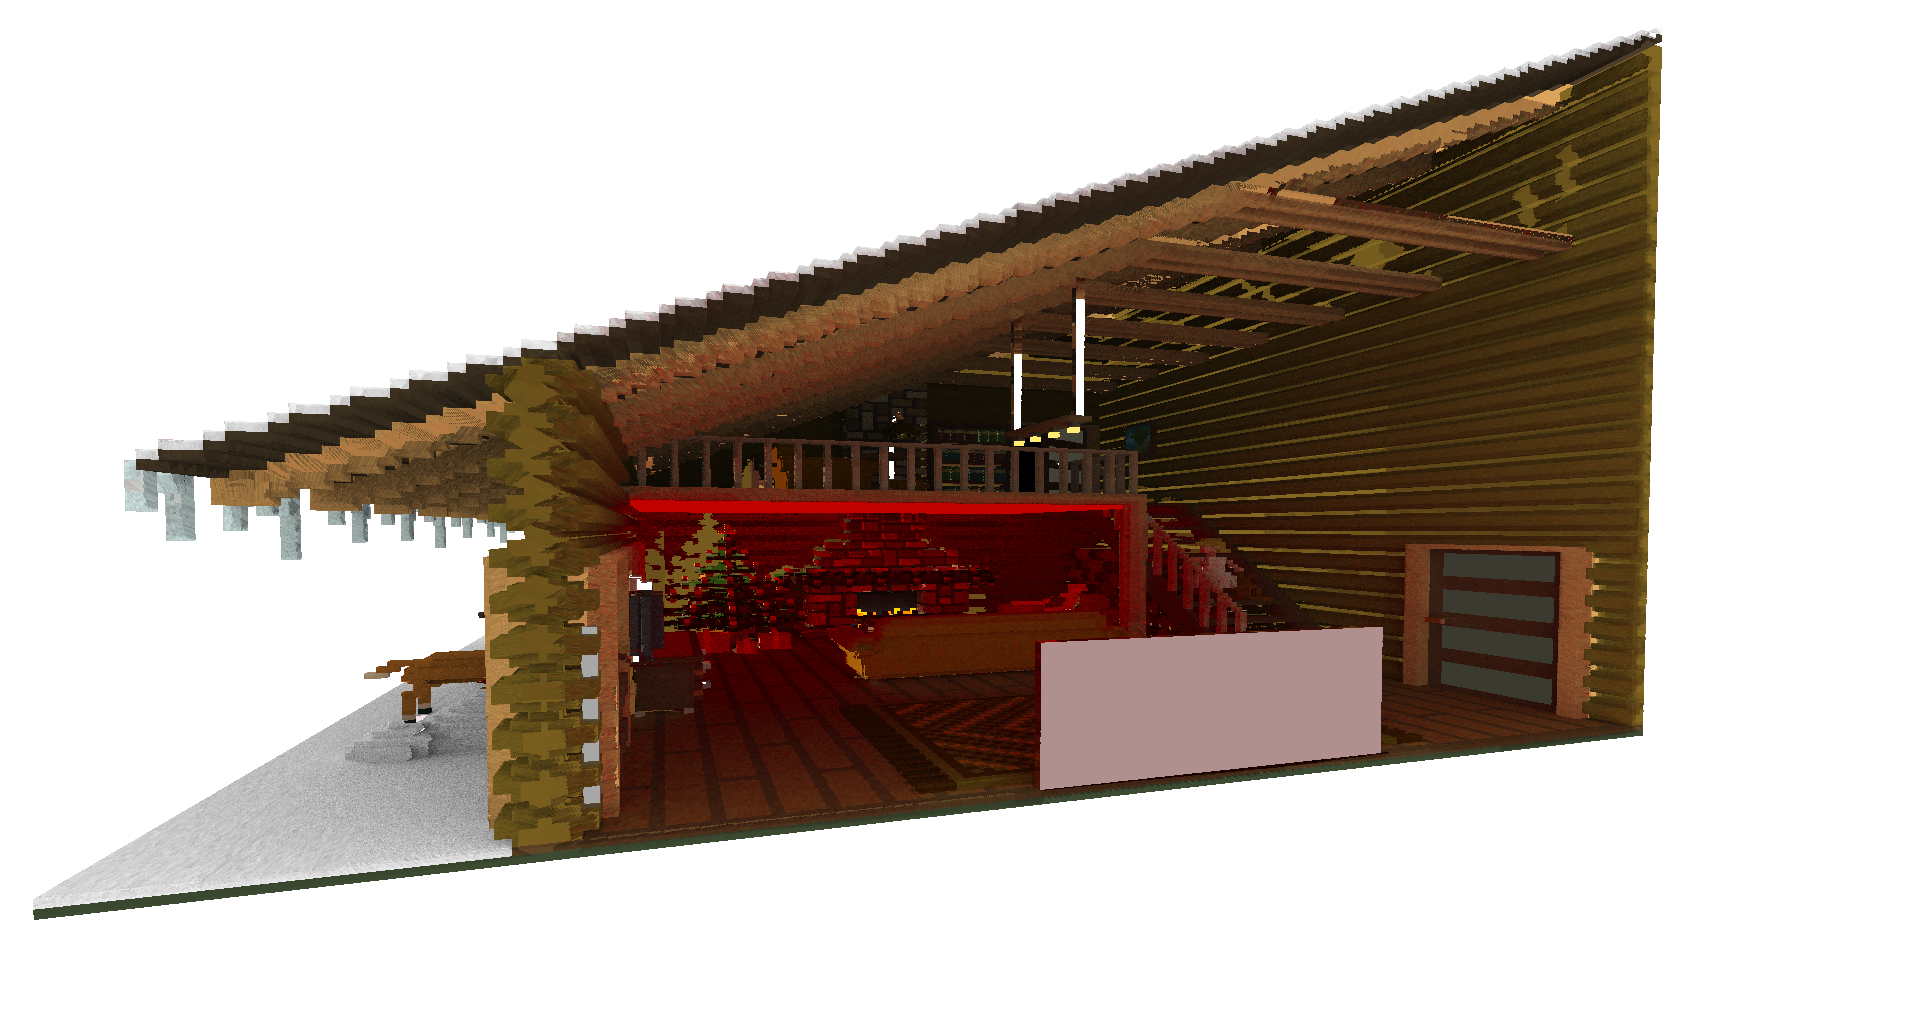
\includegraphics[width=\textwidth]{img/render1.png}
    \end{column}
\end{frame}

\begin{frame}\frametitle{Výsledky}
    \begin{column}{\textwidth}
        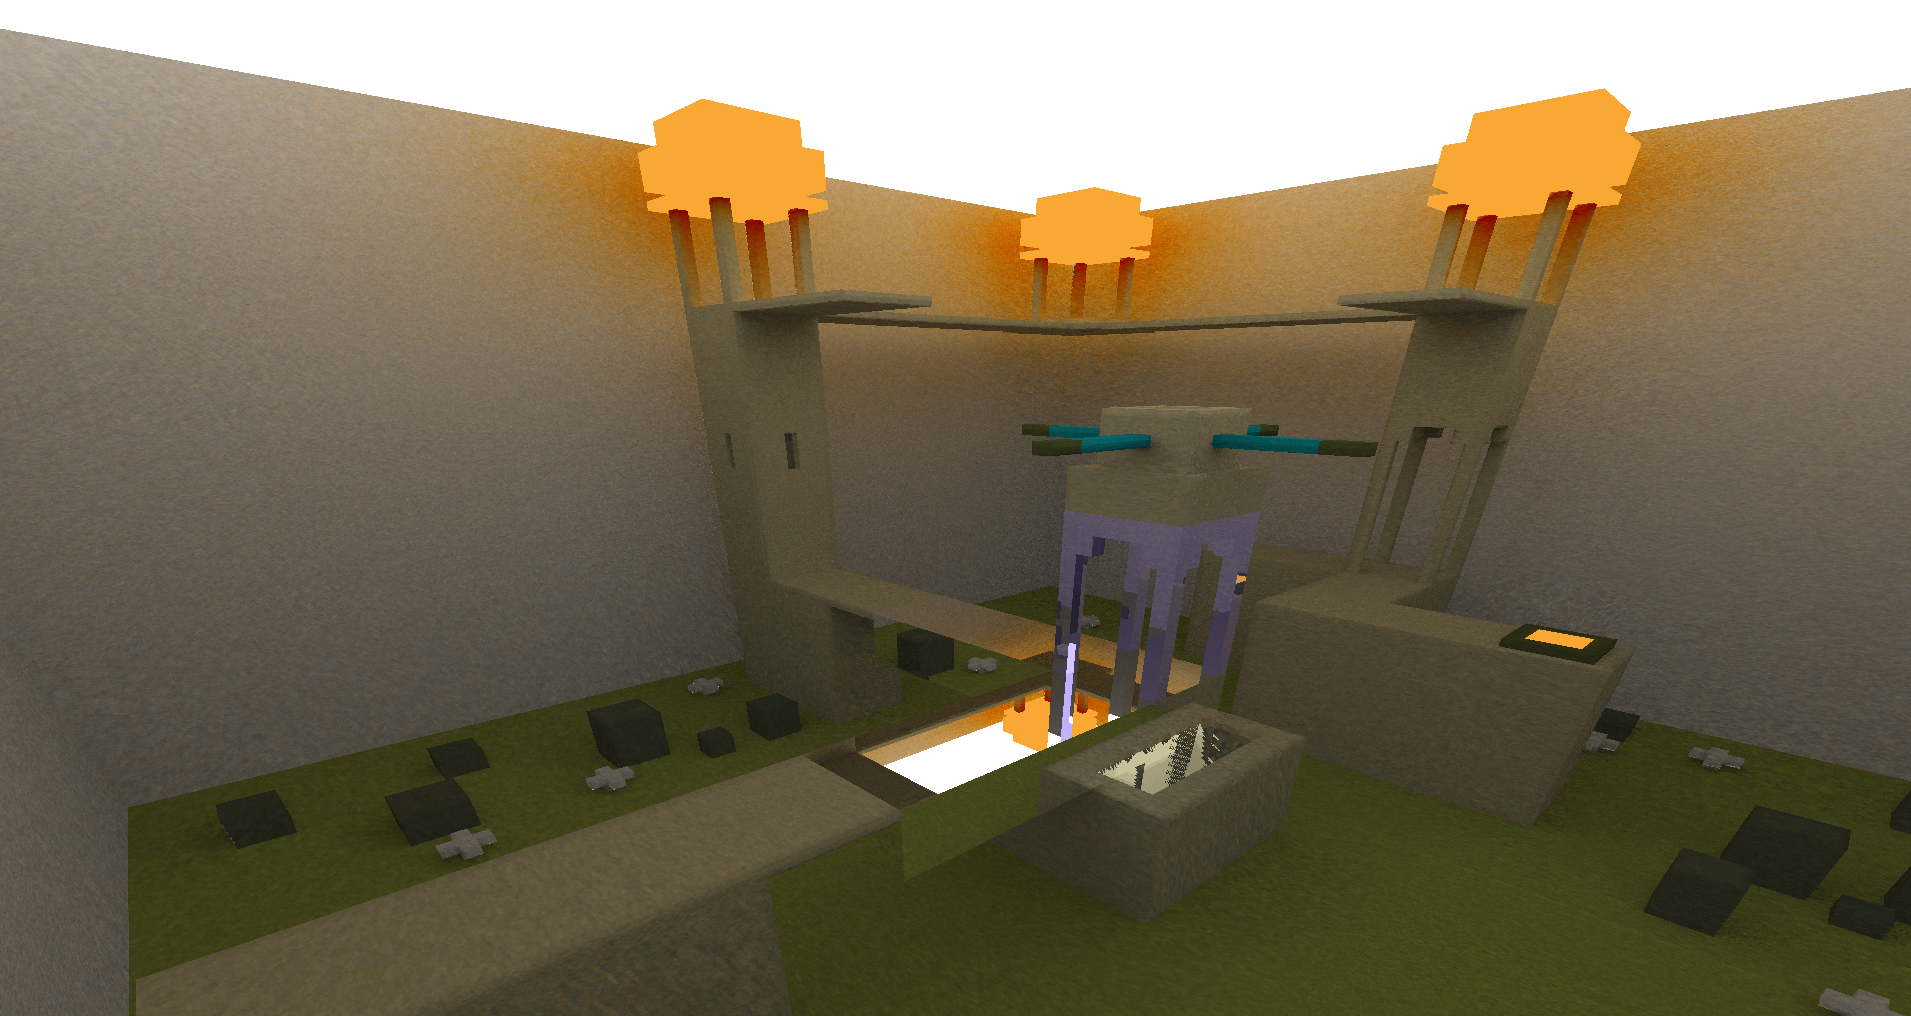
\includegraphics[width=\textwidth]{img/indirect_render_2.png}
    \end{column}
\end{frame}



\end{document}
